\documentclass[openany, longbibliography,slovene,a4paper,12pt]{article}
%\documentclass[openany,slovene,a4paper,12pt]{article}
\usepackage[a4paper,inner=3.5cm,outer=2.5cm,top=2.5cm,bottom=2.5cm]{geometry}

\usepackage{braket}
\usepackage{float}
\usepackage{afterpage}
\usepackage{graphicx}
\usepackage{amssymb}

\usepackage[tbtags]{amsmath}
\usepackage[T1]{fontenc}
\graphicspath{{../slike/}{../slike_vezikel_z_robom/}{/home/jure/sola/magisterij/uporabljene_slike/}
{../eps_pdf/}}
\DeclareGraphicsExtensions{.eps,.jpeg,.png,.gif,.pdf}
\usepackage[outdir=./slike/]{epstopdf}
\epstopdfsetup{
	suffix=,
}
\usepackage[multidot]{grffile}

% \usepackage[slovene]{babel}      % slovenski delilni vzorci (!)
% \usepackage[english]{babel}
\usepackage[utf8]{inputenc}
\usepackage{makeidx}
\usepackage{enumerate}
\usepackage{caption}
\usepackage{subcaption}
\usepackage[tbtags]{mathtools}
\usepackage{wrapfig}

\usepackage[section]{placeins}

\usepackage[hyphens,spaces,obeyspaces]{url}
\usepackage{breakurl}
%\usepackage{refcheck}


\usepackage{ragged2e}
\edef\UrlBreaks{\do\-\UrlBreaks}

\usepackage{makeidx}
\pagestyle{headings}
\makeindex
\usepackage{fancyhdr}
\usepackage[titletoc,title]{appendix}


\usepackage[sort, numbers]{natbib}
\usepackage[pdfa]{hyperref}
\usepackage[x-1a]{pdfx}
\usepackage{pdfpages}
\usepackage{breqn}


\DeclareMathOperator{\arcsinh}{arcsinh}

\def\epsfg#1#2{\epsfig{file=#1.eps,width=#2}}
\def\legendamp#1#2{\vbox{\hsize=#1\caption{\small #2}}}

\setcounter{topnumber}{4}
\setcounter{bottomnumber}{4}
\setcounter{totalnumber}{5}
\renewcommand{\topfraction}{0.99}
\renewcommand{\bottomfraction}{0.99}
\renewcommand{\textfraction}{0.0}
\setlength{\tabcolsep}{10pt}
\renewcommand{\arraystretch}{1.5}

\def\bi#1{\hbox{\boldmath{$#1$}}}
\let\oldvec\vec
\def\vec#1{\mbox{\boldmath$#1$}}
\def\pol{{\textstyle{1\over2}}}
\def\svec#1{\mbox{{\scriptsize \boldmath$#1$}}}

\newcommand{\dif}{\mathrm{d}}
\usepackage{xparse}
\DeclareDocumentCommand{\myint}{o m o o}  
{%
	\int \IfValueT{#1}{#1} \dif #2 \IfValueT{#3}{\dif#3} \IfValueT{#4}{\dif#4}
}
\newcommand{\Alpha}{A}
\newcommand{\Beta}{B}
\newcommand{\Epsilon}{E}
\newcommand{\Kappa}{K}


\begin{document}
%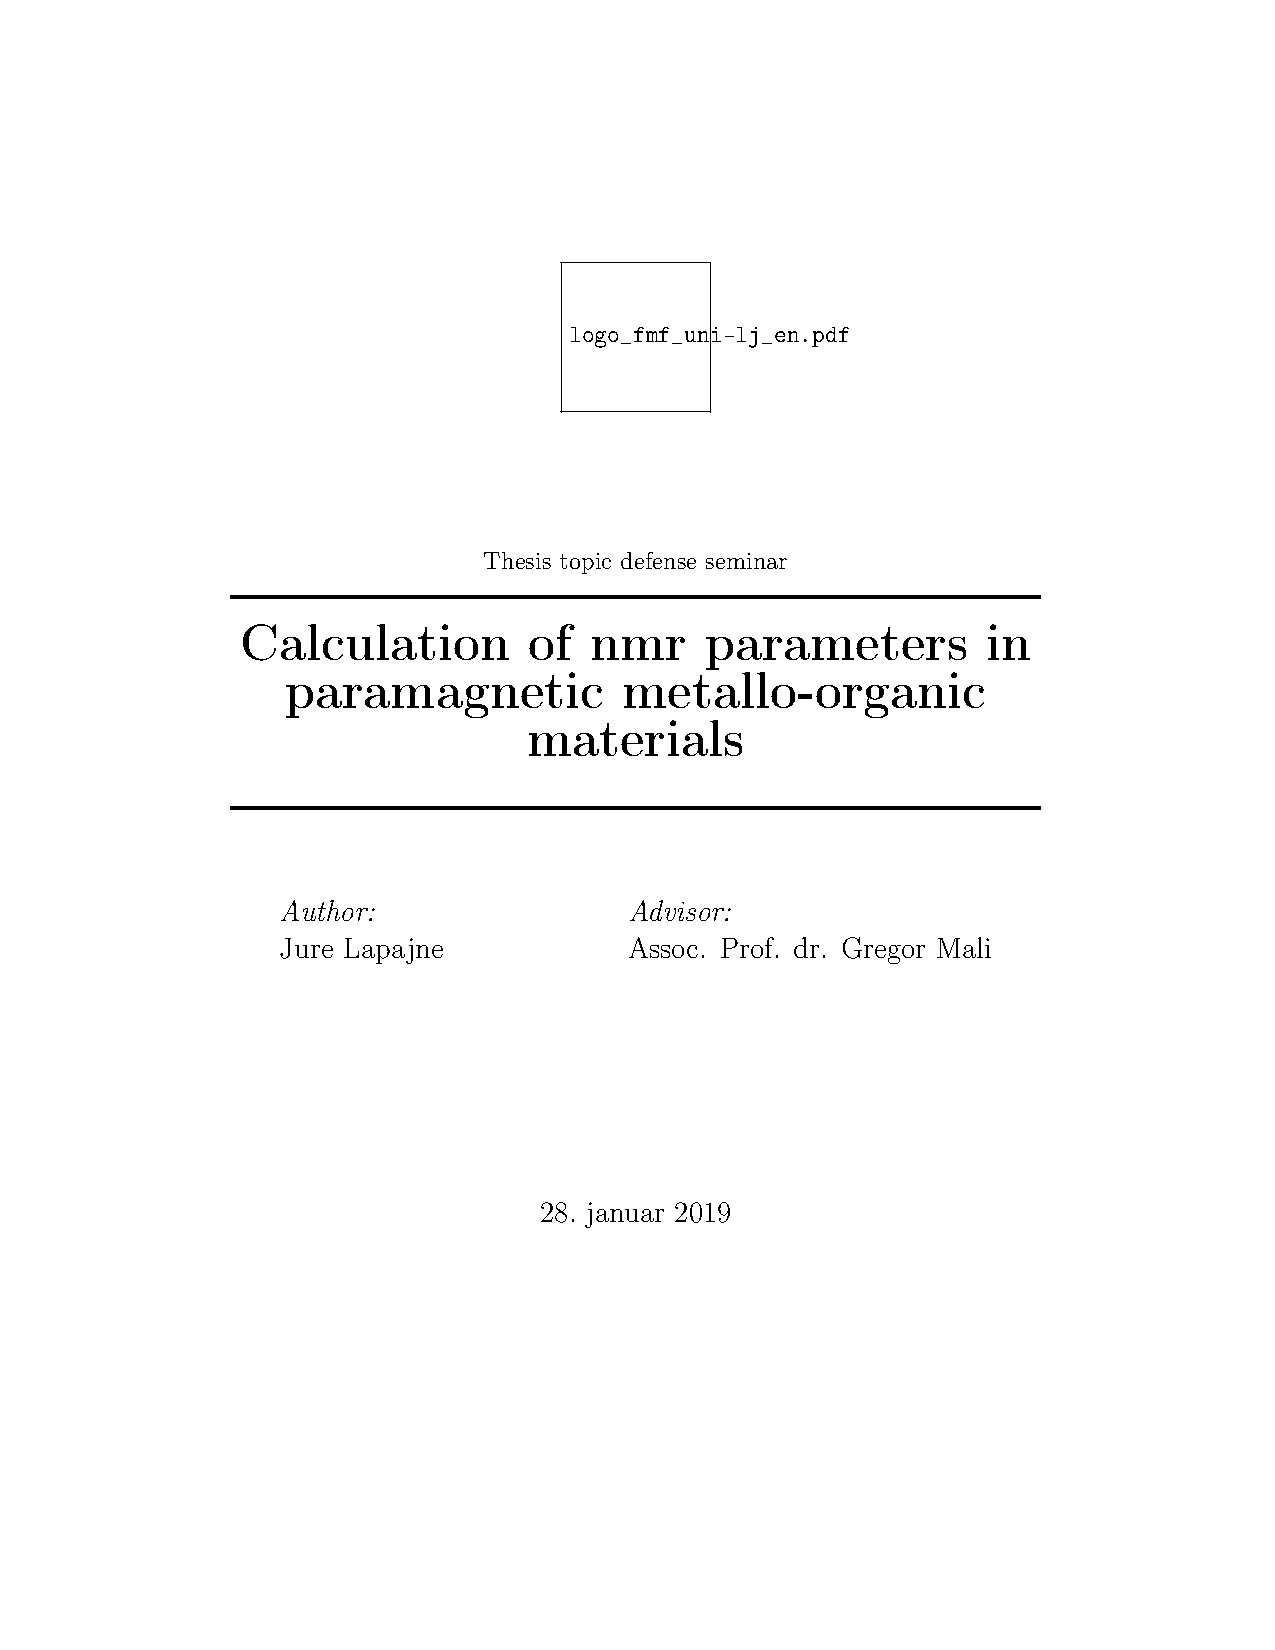
\includepdf{naslovna.pdf}


\section{Introduction}

Metal-organic frameworks or MOFs are materials consisting of one or multiple
central metallic ions and surrounding organic ligands.  They are crystalline
materials with very high porosity. Internal surface area in some cases exceeds
6000 $\mathrm{m}^2/{g}$ \cite{introd_to_metal_organ_frameworks}. Thanks to their
chemical properties they are widely used in the fields of biochemistry,
catalysis and electrochemistry. They are especially useful in clean energy
applications, as storage for gasses (eg. hydrogen) or energy through
adsorption / desorption process \cite{introd_to_metal_organ_frameworks}. They can
also be used as gas separation medium, as second harmonic generators in
nonlinear optics, some of them also display interesting ferroelectric
properties. Their usage is so broad thanks to numerous combinations of metallic
ions and organic ligands  \cite{introd_to_metal_organ_frameworks,
  Assignment_of_Solid_State}. Many MOFs contain unpaired electrons. Ions such as Cu(II), Ni(II) have unpaired electron(s) in their $d$ orbitals and one can clearly see their
 effects on $^{13}C$ and $^{1}H$ NMR  spectra, one of the most common tools for
 characterization of the molecular and electronic structure of organic
 molecules.

 Materials presented in this work are paramagnetic. This means they exhibit weak
 attraction to the external magnetic field, which is a consequence of unpaired
 electrons in their structure. The effects of the latter are easily recognized
 in NMR spectra by the large paramagnetic shifts they cause
 \cite{Dft_Investigation_of_the_Effect_of_Spin_Orbit}. Picture \ref{mof_spectre}
 shows a spectre of MOF called HKUST-1. One can observe a large shift at around
 800 ppm caused by unpaired electrons in molecule.


 \begin{figure}
   \centering
      \begin{subfigure}[b]{0.5\textwidth}
  \centering
  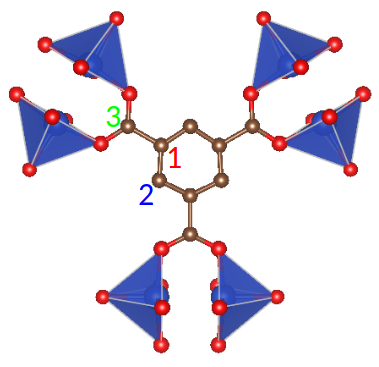
\includegraphics[width=0.65\textwidth]{hkust_molekula_placeholder.png}.
  \caption{}
  \label{mof_molecule}
\end{subfigure}%
   \begin{subfigure}[b]{0.5\textwidth}
  \centering
  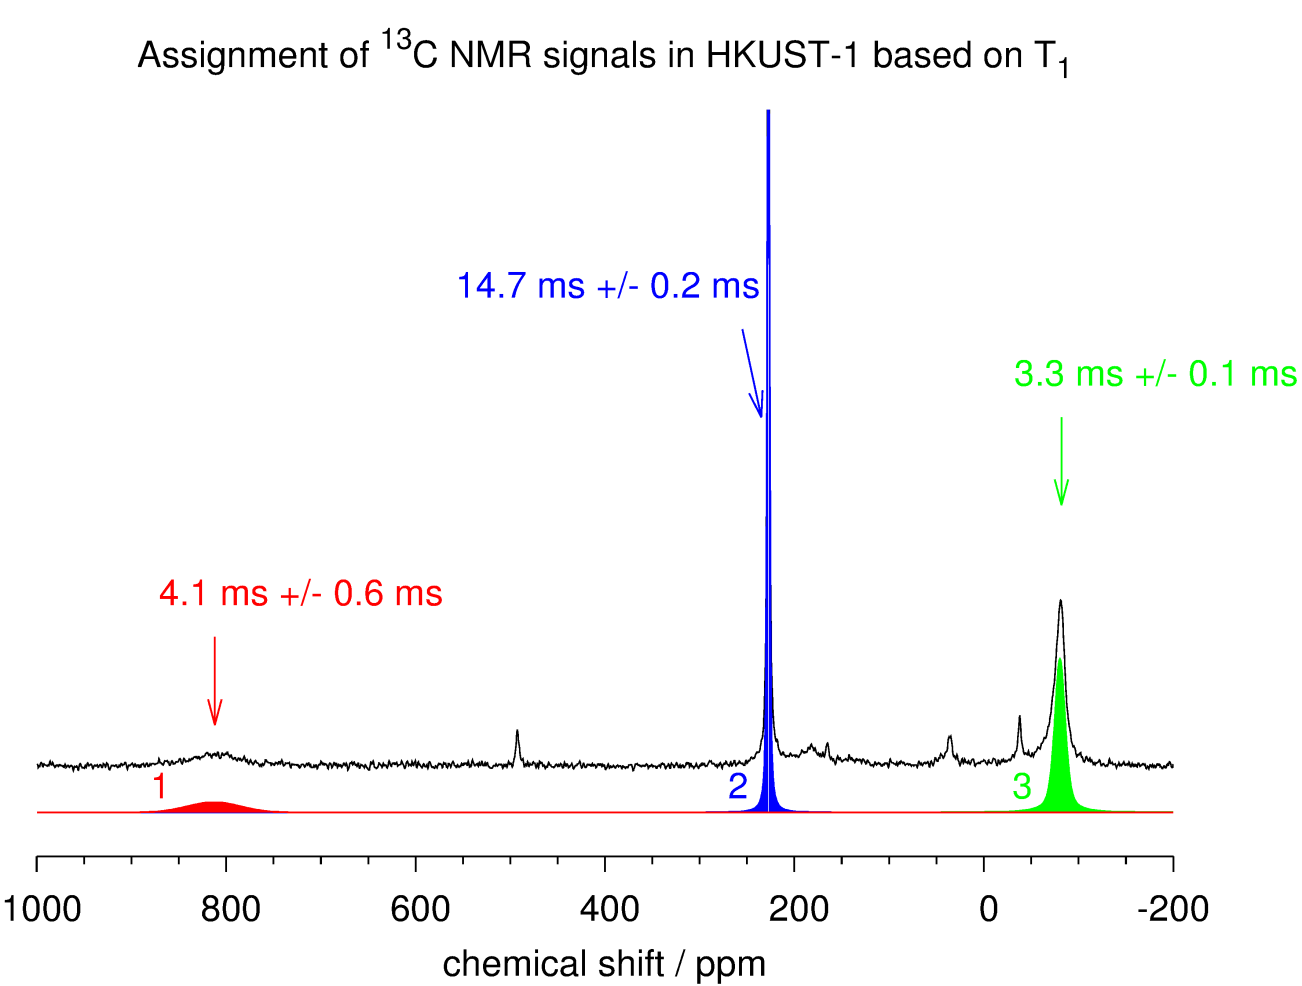
\includegraphics[width=0.9\textwidth]{hkust_spekter.png}.
  \caption{}
\end{subfigure}
  \caption{ An example of MOF named HKUST-1. It is a crystalline
    material. Image (a) depicts a part of the crystaline structure which is used for calculation of
    NMR parameters of atoms marked with 1, 2 and 3. (b) $^{13}\mathrm{C}$-NMR
    spectra of atoms marked on scheme (a).
  }
  \label{mof_spectre}
  \end{figure}

 NMR spectra of organic materials usually feature chemical shifts caused by
 induced currents which in turn, are caused by external magnetic field
 \cite{chemic_shift_tensor_review}. In paramagnetic materials, this is not the
 only contribution to the total shifts visible in spectra. An important
 interaction, not present in  diamagnetic materials, is interaction between
 unpaired electrons and nuclei
 \cite{Dft_Investigation_of_the_Effect_of_Spin_Orbit}.
 Such interaction can cause large paramagnetic
 shifts also called hyperfine shifts. Typical for such spectra are also widened
 spectral lines. These large shifts make interpretation of spectra more difficult
 \cite{Dft_Investigation_of_the_Effect_of_Spin_Orbit}. A useful tool to help
 with the interpretation are first-principle quantum calculations. Large growth
 of computational power in recent years have enabled more accurate calculations
 and calculations performed on a more complex systems. Development of
 computational tools have also enabled computations of shielding and hyperfine
 tensors. The former is responsible for large shifts caused by unpaired
 electrons whereas the latter is present in all molecules and is caused by
 currents induced by external magentic field. Although most common computational
 packages offer computations of these two tensors, total chemical shifts for
 paramagnetic materials / MOFs have not yet been systematically tested and
 documented in the literature.

\section{Calculation of electronic wavefunction}
Accurate calculation of electronic structure has always been a challenge. It
quickly became apparent that direct use of Schr{\"o}dinger equation is not a
realistic prospect, except for some small
molecules, as the time consumed to solve it grows exponentially
\cite{nobel_lecture} as a function of electron
number at a given accuracy level. With the development of computers, different
numerical approximations for computation of electronic wave function and
optimization of molecular structure have emerged. One of the most successful methods has been density functional theory
(DFT from now on), which has been known for roughly 50 years \cite{nobel_lecture}. Through the years DFT has evolved and today it represents one of the main tools for calculation of electronic structure especially for complex molecules and crystals.

\subsection{Hamiltonian}
The first step in formulation of the problem is to define hamiltonian which
describes the motion of nuclei and electrons. Non-relativistic hamiltonian
describing the interaction of  nuclei and electrons can be written as follows:
\begin{equation} \label{full_hamiltonian}
\hat H= \hat T_n + \hat  T_e + \hat  W_{n-n} + \hat W_{e-e} + \hat W_{n-e} + \hat V_{ext},
\end{equation}
where $T_n$ and $T_e$ are kinetic energies of nuclei and electrons respectively,
$W_{n-n}$, $W_{e-e}$ and $W_{e-n}$ represent nuclei-nuclei, electron-electron
and electron-nuclei interaction terms. $V_{ext}$ is strictly multiplicative
external potential. Ground state of such a system is given by the solution of
the time independent Schr{\"o}dinger equation:
\begin{equation} \label{ham_solution}
\hat H \ket { \psi_0 } = \epsilon_0 \ket{ \psi_0 },
\end{equation} 
where index $0$ denotes the solution with the lowest energy. In general $\psi_0$
depends on $3N$ coordinates, where $N$ is the total number of particles. This means
that systems with more than e.g. 10 atoms are very computationally
demanding. It is common practice to reduce the dimensionality of the problem by employing
Born-Oppenheimer approximation in which the motion of nuclei is separated from
the motion of electrons, sometimes their positions are even fixed
\cite{advanced_course, nobel_lecture}. Thus, from now on, we will
restrict ourselves to hamiltonians describing only the motion of electrons:
\begin{equation} \label{electron_hamiltonian}
\hat H=  \hat  T_e  + \hat W_{e-e} + \hat W_{n-e} + \hat V_{ext}.
\end{equation}
The number of electrons $N$ for a small molecules, like water, is of the order
$\sim 10$. In medium sized molecules with $\sim 50-100$ atoms, the number can
grow to a few hundred, while in large molecules, like proteins, the number can
grow into thousands and ten-thousands \cite{ab_initio_nmr_spect_molec}. As one can imagine, solving a system of
coupled differential equations with so large number of coordinates ($3N$) is
computationally an almost impossible task.
This is the reason for development of approaches which, while still being
sufficiently accurate, offer shorter computational times. DFT represents one of
the most successful methods for solving such systems.

\subsection{Density functional theory - DFT}
DFT allows us to replaces all electron wave function with
electron density and effectively reduce the problem to a single electron problem.
The core of DFT lies in Kohn-Sham theorems. These two theorems
prove that stationary many-electron systems are fully characterized by their
ground state electron density. This means that given a group of electrons, one
only has to know ground state electron density to be able to tell all the other
properties of this group of electrons \cite{nobel_lecture}. For non-degenerate
cases, the latter is uniquely determined by the ground state many-electron wave
function, which in turn is uniquely determined by the external potential.
Uniquely determined means that there exists bijection between the set of
potentials, which yield non-degenerate ground states, the set of ground state
wave functions and ground state electron densities. The bijection is depicted on
the figure \ref{bijection}. The figure denotes mentioned sets as $\mathcal V$,
$\mathcal G$ and $\mathcal N$.

\begin{figure}[!ht]
  \centering
  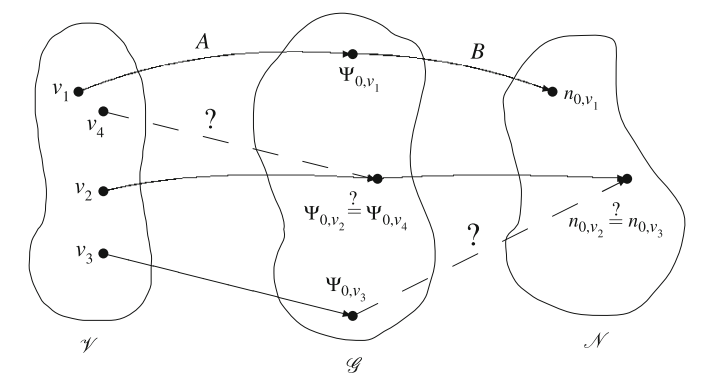
\includegraphics[width=0.6\textwidth]{bijekcija_med_v_psi_n.png}.
  \caption{Bijection between the set of potentials, the set of their corresponding ground
    states and the set of ground state densities. Existance of such bijection is proven by
    Kohn-Sham theorems and ensures that many-particle system is
    uniquely determined by its ground state particle
    density~\cite{advanced_course}.}
  \label{bijection}
\end{figure}

Since there exists bijection between ground state wave functions and ground
state densities, one can formally rewrite ground state wave function as
functional of ground state electron density:
\begin{equation}
  \ket{\psi'_0} =  \ket{\Psi[n'_0]}
  \end{equation}
and using above formula one can also rewrite operators in terms of ground state
density. As an example, let us rewrite ground state energy as functional of
ground state electron density:
\begin{equation} \label{hamiltonian_density}
  E[n_0] = \bra{\Psi[n_0]}\hat H \ket{\Psi[n_0]},
  \end{equation}
for which one can find minimum energy principle: $E[n_0]<E[n]$ whenever $n(\vec r)$
belongs to $\mathcal N$. This is an obvious consequence of wave function functional
$\ket{\Psi [n]}$, which is only defined for densities which are in $\mathcal N$.
Thus, one has to ask himself whether every nonegative normalizable function
$n(\vec r)$ is in $\mathcal N$.  The answer is no. A density from $\mathcal N$
has a corresponding potential $V_{ext}$ such that it minimizes energy functional
of the form \ref{hamiltonian_density} and consequently they are called V-representable densities.
In practice, this is not really important. The reason for this is the discretization of space
into grid points. On final grid for any strictly positive electron density
($n(\vec r) > 0$) belongs to $\mathcal N$ \cite{advanced_course}.


  \section{DFT in practice}
Kohn-Sham theorems unfortunately tell nothing about the explicit dependence of
energy functional on density. Nonetheless, we would still like to use Kohn-Sham
theorems, to construct numerical scheme in which electron density has the central
role. From now on will concentrate on construction of a suitable DFT scheme and
finding energy functional $E[n(\vec r)]$, which should approximate the given
system as well as possible.
  
  \subsection{Kohn-Sham equations}
  Kohn-Sham (KS) equations represent a standard and most common approach to DFT.
  They are based on energy functional dependent only on electron density $n(\vec
  r)$. To introduce them in an understandable and consistent fashion, let's start with a non-interacting system. 
 
\subsection{Noninteracting system}
Hamiltonian of $N$-electron non-interacting system can be written in the
following way:
 \begin{equation} \label{noninteracting_H}
   \hat H =\hat  T + \hat V_{ext}, 
 \end{equation}
 where $V_{ext}$ is an external potential of multiplicative nature. It is well
 known that the solution to this problem can be written in the form of Slater determinant:

 \[
      \frac{1}{\sqrt{N!}}\det 
   \begin{bmatrix}
   \phi_{1}(\vec r_1, \sigma_1) & \phi_{2}(\vec r_1, \sigma_1) & \phi_{3}(\vec
   r_1, \sigma_1) & \dots & \phi_{N}(\vec r_1, \sigma_1) \\
    \phi_{1}(\vec r_2, \sigma_2) & \phi_{2}(\vec r_2, \sigma_2) & \phi_{3}(\vec
    r_2, \sigma_2) & \dots & \phi_{N}(\vec r_2, \sigma_2) \\
    \vdots & \vdots & \vdots & \ddots & \vdots \\
     \phi_{1}(\vec r_N, \sigma_N) & \phi_{2}(\vec r_N, \sigma_N) & \phi_{3}(\vec r_N, \sigma_N) & \dots & \phi_{N}(\vec r_N, \sigma_N) \\
\end{bmatrix},
\]
 which, when inserted into equation (\ref{noninteracting_H}) effectively produces
a set of single electron problems:
 \begin{equation}
   \left(-\frac{\hbar^2}{2m}\nabla^2 + \hat V_{ext}(\vec r)\right) \phi_i (\vec r) = \epsilon_i \phi_i(\vec r).
 \end{equation}
 Thus, using slater determinant, we have effectively converted many electron
 problem with $3N$ coordinates to a single electron problem. Of course the
 electrons in this case do not feel each other and motion of each electron
 should not depend on other electrons, so such a breakdown is completely natural
 (except for Pauli principle, which is already built into the Slater determinant).
 
 The ground state of such a system is obtained by putting pairs of electrons
 into each of  $N/2$ lowest states. Calculation of kinetic energy and
 electron density for such a system is straight forward. As we can see,
 using Slater  determinant as ansatz for the solution of noninteracting
 hamiltonian offers simple expressions for ground state wavefunction, kinetic
 energy and electron density  calculation. Electron density corresponding to
 such a wave function can be written using the following expression:
 \begin{equation} \label{KS_density}
   n_0(\vec r) = \sum_{\sigma=\uparrow,\downarrow}\sum_i\Theta(\epsilon_F-\epsilon_i)|\phi_i(\vec r, \sigma)|^2,
 \end{equation}
 where $\Theta$ is a Heavyside function.
 The density of electrons is just a sum over all occupied orbitals. Now let's
 remember Kohn-Sham theorems, which state that ground state density is unique
 functional of the ground state wave function:
 \begin{equation}
   \ket{\psi(\vec r)}= \ket{\Psi[n(\vec r)]}.
 \end{equation}
 One can show that there exists an even stronger connection; every $\phi_i$ is a
 uniquely determined by ground state density. One can see this by considering a single electron problem using the same potential $V_{ext}$ as found in eq.
 (\ref{noninteracting_H}) and then gradually adding electrons, thus:
 \begin{equation}
   \ket{\phi_i(\vec r)}= \ket{\Phi_i[n(\vec r)]}.
 \end{equation}
 Using this relations we can define HK functional:
 \begin{equation}
   E_s[n(\vec r)] = \bra{\Psi[n(\vec r)]}T \ket{\Psi(n(\vec r))} + \int n(\vec r) V_{ext}(\vec r)  \dif \vec r,
   \end{equation}
 where
\begin{equation} \label{KS_kinetic_term}
   T[n(\vec r)] = \sum_i\Theta(\epsilon_F-\epsilon_i)  \sum_{\sigma=\uparrow,\downarrow}\int \phi^*_\sigma(\vec r)\frac{-i\hbar\nabla^2}{2m}\phi_\sigma(\vec r),
 \end{equation}
 where we have implicitly used $\ket{\phi_i(\vec r)} = \ket{ \Phi_i[n(\vec r)] }$.
 In practice this in not necessary, since functions $\phi(\vec r)$ are known.
 
Now we would like to use a similar construction to solve hamiltonian
\ref{hamiltonian_density}. Using solution ansatz in the form of Slater
determinant offers straight forward calculation of kinetic energy and electron
density. Using Slater determinant leads to differential equations for $\phi_k$
wavefunctions. Modern computational packages instead of solving differential
equations use large sets of basis functions, which in the end lead to
an eigenvalue problem. Solution is then given by populating
lowest energy orbitals until all electrons are allocated.

To solve interacting system using DFT one relies on the fact, that for every
interacting hamiltonian with ground state density $n_0$, there exists
noninteracting hamilotnian with exactly the same ground state density \cite{advanced_course}.
This fact still does not tell us what kind of external potential
one should use to produce the same electron density.

Intuitively, one would expect that potential belonging to effective single
electron hamiltonian should reflect the properties, geometry and potentials found
in a given interacting system. Hamiltonian naturally contains kinetic energy
term, but it should also somehow contain inter particle interactions. Usually
Kohn-Sham hamiltonian consists of kinetic energy term, Hartree inter particle
interaction, external potential and exchange-correlation functional \cite{advanced_course}:
\begin{equation} \label{KS_system}
  E[n(\vec r)]=T[n(\vec r)] + E_H[n(\vec r)] + E_{ext}[n(\vec r)] + E_{xc}[n(\vec r)].
\end{equation}
Hartree term accounts for Coulomb repulsion:
\begin{equation} \label{hartree_term1}
  E_H[n(\vec r)] = \int\frac{ n(\vec r) n(\vec r')}{|\vec r -  \vec r'|} \dif \vec r' \dif \vec r.
\end{equation}
The above expression is not the same as the one we get from Hartree-Fock
equations and includes self-repulsion. DFT treats exchange term, also arising
from Coluomb potential, separately. Computational packages often employ different
approximation and optimizations for shorter calculation of this term \cite{orca}.
Functional belonging to external potential is well known: 
\begin{equation} \label{ext_potential_functional}
  E_{ext}[n(\vec r)] = \int n(\vec r) V_{ext}(\vec r) \dif \vec r.
\end{equation}
Unfortunately exchange-correlation functional is much less well known. It is
defined by the equation (\ref{KS_system}) and contains all the inter-particle
interactions not contained in $T[n(\vec r)]$ and $ E_H[n(\vec r)]$. It is
common to divide $E_{xc}[n(\vec r)]$ into exchange $E_x[n(\vec r)]$ and
correlation $E_c[n(\vec r)]$ part. The former is defined in such a way that
Hartree-Fock ground state density and energy are reproduced, if correlation part
is neglected. This is achieved if exchange part of functional has exactly the
opposite contribution as excessive hartree term in KS equations: 

\begin{equation}
  E_{x}[n(\vec r)]=-\frac{1}{2}\sum_{k,l}\Theta(\epsilon_F-\epsilon_k)\Theta(\epsilon_F-\epsilon_l)\int \dif \vec{r} \dif \vec{r'}\phi^*_k(\vec r, \sigma)\phi_l(\vec{r}, \sigma)w(\vec{r},\vec{r'})\phi^*_l(\vec{r'}, \sigma')\phi_k(\vec{r'}, \sigma')
\end{equation}
The most important contribution of $E_{x}[n(\vec r)]$ is cancellation of
self-repulsion. This term is commonly called exact exchange and is not always
used in DFT calculations. Exchange functionals based only on
electron density are often employed and they do not manage to completely cancel
self-repulsion terms. We will take a closer look at them in the following chapter.
Correlation term is more difficult to derive and we will not dwell deeper into
it. Instead let's have a look at how KS equations are actually solved.

Our goal is to minimize energy of the form (\ref{KS_system}) using Slater
determinant as ansatz for many electron system and density calculation. By
considering (\ref{ext_potential_functional}) and (\ref{KS_kinetic_term}) one can
write KS equation:  
\begin{equation}
  \left( \hat T + V_{ext} + E_H[n(\vec r)]  + E_{xc}[n(\vec r)] \right) \ket \phi_i =  \epsilon_i \ket{\phi_i},  
\end {equation}
where density $n(\vec r)$  has to be calculated according to equation
(\ref{KS_density}). They are usually determined by inserting ansatz in the
form of gaussian basis functions from which one can
then construct correct single electron states. Multiplying equation by $\bra
\phi_j$ from the left side yields generalized eigenvalue problem:
\begin{equation}
  \bra {\phi_j} \left( \hat T + V_{ext}(\vec r) + E_H[n(\vec r)]  + E_{xc}[n(\vec r)] \right) \ket{\phi_i} =  \epsilon_i \braket{ \phi_j |\phi_i }.
\end {equation}

System obviously has to be solved in a self consistent fashion
(fig. \ref{self_consistent_scheme}). One starts with the positioning of nuclei into
desired positions and construction of nuclei potentials. In parallel with the
last step starting electron orbitals $\phi^{(0)}_i$ are constructed. Usually they are written
as a series of Gaussian functions. Electron density $n^0$ can then be quickly
calculated from constructed orbitals. After that one
calculates functionals $E_H[n(\vec r)]$ and $E_{xc}[n(\vec r)]$. In the next step
equations are solved. The solution are new orbitals $\phi_i^{(1)}$  and from
them, the new density $n^{(1)}$ is calculated. The latter is then used to construct new $E_H[n(\vec r)]$ and $E_{xc}[n(\vec r)]$ which are again used to
solve KS equation from which one gets new orbitals $\phi_i^{(2)}$. The procedure is
repeated until the change in density or energy is small enough. 


\begin{figure}
  \centering
  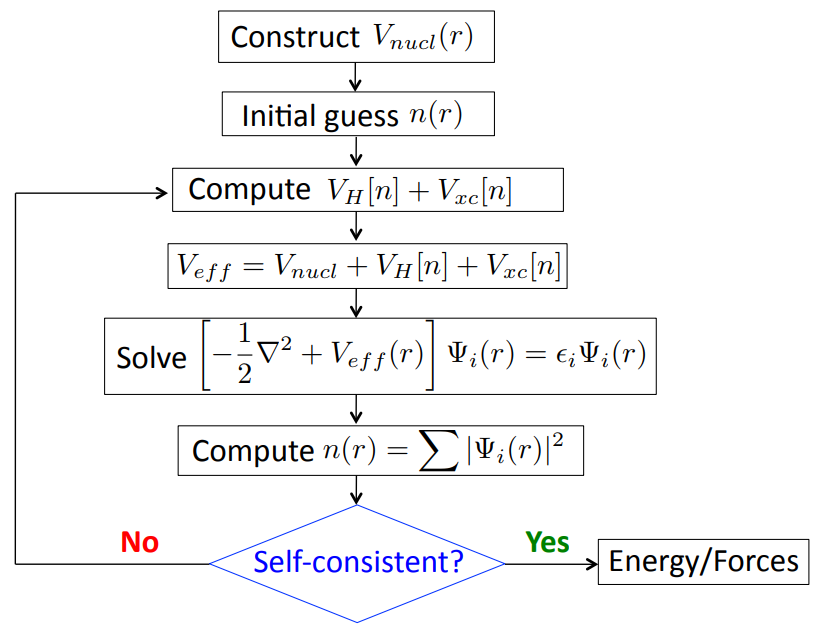
\includegraphics[width=0.65\textwidth]{self_consistent_scheme.png}.
  \caption{Self consistent scheme depicting the procedure in which Kohn Sham
    equations are solved. One starts with the positioning of nuclei into
    desired positions. The next step is to construct potential of nuclei and in
    parallel one can also construct starting approximation for electronic wave
    function. The latter is then used for constructing all other functionals of
    density. After all functionals have been established one can solve KS
    equations, construct new density and repeat the described procedure until
    the change in density is not small enough \cite{qe_tutorial}.
  }
  \label{self_consistent_scheme}
\end{figure}

When given a certain system, functionals $T$, $E_H$ and $V_{ext}$ are precisely
determined. $E_{xc}$ is not. It is thus the determining factor for how well the KS
equations describe our system. We will present various functionals used today in
one of the next chapters.

\subsubsection{Degenerate ground state}
So far we have talked little about the problem of degeneracy of KS states. In
general degeneracy is not a problem, except at Fermi level. When there are more
KS states than there are electrons, several possible ground states and thus also
electron densities can be constructed. In such cases density matrix arising from
several Slater determinants is constructed \cite{advanced_course}:
\begin{equation}
  \hat D = \sum_i d_i\ket{\Phi_i} \bra{\Phi_i}.
  \end{equation}
Density belonging to such ground state is just a weighted sum of densities
corresponding to each Slater determinant $n(\vec r)=\sum_id_in_i(\vec r)$, where
$n_i(\vec r)=\sum_j|\phi_{ij}(\vec r)|^2$. Index $i$ runs over all possible
Slater determinants one can construct from given degenerate states and index $j$
runs over all states in each Slater determinant. The sum of coefficients $d_k$
is the trace of density matrix and has to be $1$. The choice of coefficients
$d_k$ is not trivial. They have to be constructed in such a way that the new
electron density does not break degeneracy. When a new degenerate state emerges in
scf procedure (fig. \ref{self_consistent_scheme}), it may significantly affect
electron density and resulting potentials and consequently break or destroy
convergence of the procedure. An example is a boron atom where 2p orbitals are
degenerate. Only the choice of $d_{2p^0}=d_{2p^{-1}}=d_{2p^1}=1/3$ leads to spherically symmetric potential and preservation of degeneracy\cite{advanced_course}.

\subsection{Exchange and correlation functionals}
Exchange and correlation functionals are functionals which try to account for
exchange and correlation interactions between electrons. They can be of
different forms and in general one can roughly divide them into four groups
\cite{challenges_den_fun_theor, presc_desig_selec_densit_funct_approx}: Lda, Gga, meta-Gga and Hybrid functionals.
The first three groups all have in common that they explicitly depend on density
of electrons. This causes a self-interaction error, which causes excessive
delocalization of electrons. As a solution to these problems hybrid
functionals, which contain exact Hartree-Fock exchange, have been proposed.


\begin{figure}[!ht]
  \centering
  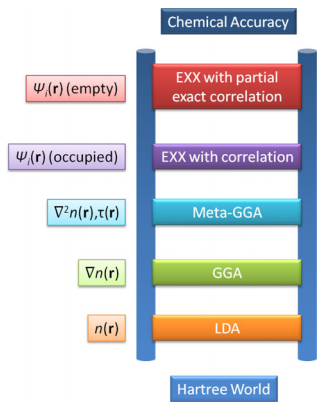
\includegraphics[width=0.4\textwidth]{jacobs_functional_ladder_ver2.png}.
  \caption{Jacob’s ladder of exchange-correlation functional approximations
    employed in DFT calculations. Hartree world represents starting level where only
    weak interparticle interaction is present. Lda approxiamtion covers
    functionals which depend only on electron density. Gga additionally depends
    on gradient of electron density, while mega-gga incorporates higher order
    derivatives of electron density and in some cases even kinetic energy of
    orbitals ($\tau$). Hyper-gga functionals, also called hybrid functionals,
    stage represents functionals which contain exact exchange calculation (i.e.
    the one found in Hartree-Fock method). The last level utilizes all Kohn-Sham
    orbitals to calculate correlation and exchange interaction. This level also
    accounts for VdW interaction, which is caused by charge fluctuations and is
    not accounted for in previous stages \cite{How_theo_simul_can_address}.
  }
  \label{ladder}
\end{figure}

\subsubsection{Lda}
Local density approximation (lda) are functionals which depend only on
 electron density \cite{challenges_den_fun_theor, presc_desig_selec_densit_funct_approx}.
First functional of such form dates back into
the year 1930, when the exchange interaction for uniform gas was discovered
\cite{challenges_den_fun_theor} :
\begin{equation} \label{electron_gas_exchange}
E_{xc}^{lda}[n]=-\frac{3}{4}\left( \frac{3}{\pi} \right)^{1/3}\int n(\vec r)^{4/3} \dif \vec r.
\end{equation}
The correlation part has not been derived, but it is accurately known from Monte
Carlo simulations \cite{presc_desig_selec_densit_funct_approx}.
Today, there exist multiple other lda exchange--correlation functionals, but for most cases
they are not very useful. Their only advantage are short computational times.
For every other purpose gga and hybrid functionals are much better suited.

\subsubsection{Gga}
Generalized gradient approximation (gga) functionals
depend not only on electron density, but also on its gradient
\cite{challenges_den_fun_theor}. Most commonly, gga functionals are built upon (\ref{electron_gas_exchange}) \cite{challenges_den_fun_theor}:
\begin{equation}
  E_{xc}^{gga}=\int n(\vec r)^{4/3}F(x);\quad x=|\nabla n(\vec r)|/n(\vec r)^{4/3}.
\end{equation}
One of most commonly used gga functionals is PBE functional
 \cite{challenges_den_fun_theor}:
\begin{equation}
  E_{xc}^{pbe}=-\int  n(\vec r)^{4/3}\left[ \frac{3}{4}\left(\frac{3}{\pi}\right)^{1/3} + \frac{\mu s}{1+ \mu s^2/\kappa} \right]; \quad s=x/(2(3\pi/2)^{1/3}).
\end{equation}
Gga functionals offer acceptable accuracy and short computational times and are
most commonly used for approximate calculations, before starting more accurate
and more time consuming calculations using hybrid or meta-gga functionals.

\subsubsection{Meta-gga functionals}
Since gga functionals have their short commings, meta-gga functionals were formed
in belief that adding higher derivatives will improve accuracy
\cite{challenges_den_fun_theor}. Meta-gga functionals are built upon gga
functional form and add terms containing higher order derivatives of electron
density. They higher computational cost than gga functionals, but are not significantly better than gga
functionals and are thus not so popular.


\subsubsection{Hybrid functionals}
On the contrary to meta-gga functionals, hybrid functionals are much more
successful \cite{challenges_den_fun_theor}. These functionals are not a
continuation of lda, gga, meta-gga chain. Instead, they incorporate exact
Hartree-Fock exchange term \cite{challenges_den_fun_theor}:
\begin{equation}
  E^{hf}_{xc}=\sum_ {i,j,\sigma}\int\frac{\phi^*_{i\sigma}(\vec r) \phi_{j\sigma}(\vec r) \phi^*_{j\sigma}(\vec r') \phi_{i\sigma}(\vec r')}{|\vec r - \vec r'|}\dif \vec r \dif \vec r'.
\end{equation}
Such functionals do not break Kohn Sham formalism since the wave functions
$\phi_i(\vec r)$ are unique functional of densities as shown in previous
chapter.

\subsection{Van der Waals dispersion}
DFT does not take into account effects caused by charge fluctuations. These Van
der Waals effects can be taken care of with different methods.
 The most promising seems to be the so called DFT-D method
\cite{consis_accur_ab_initio_param}, which is just a sum of terms $CR^{-6}$
over all atom pairs. As it is generally known, for large distances Van der Waals
potential should decay as $R^{-6}$ and this interaction does fulfill this
condition.


\section{NMR measurements}
NMR is a technique, where one uses external magnetic field to split the energy levels of
a nuclei with a nonzero spin. However, the magnetic field does not affect only
the nuclei, but is also affects electrons. Differences in electronic structure is
what causes differences among spectra of the same element in different molecules.
Thus, using NMR, one can get the information about the environment of the
observed nucleus and electronic structure of molecule.

The standard way to measure effects of NMR parameters is to introduce shielding
tensor. A unique shielding tensor belongs to each core in a molecule. The tensor
depends only on electron density at given nucleus and has non zero values for
all nuclei featuring nonzero spin. It contains information about the currents
induced by external magnetic fields. It defined by the following equation:
\begin{equation}
  \vec B_{eff}=\vec B_{ext}(I-\underline{\underline{\sigma}}).
  \end{equation}
The tensor is not measured directly, instead one measures just a relative
deviation from some reference molecule called chemical shift:
\begin{equation}
  \underline{\underline{\delta}}= ( \underline{\underline{\sigma}}_{ref} -  \underline{\underline{\sigma}}_{sample})  (I-\underline{\underline{\sigma}}_{ref})^{-1}  \rightarrow \delta ^{iso}\approx \sigma^{iso}_{ref} -  \sigma^{iso}_{sample}.
\end{equation}
The left part of equation is the rigorous definition. More commonly, the right
part is used, which is a trace of the left side under the assumption that
$(\underline{\underline{\sigma}}_{ref})_{ij} \ll 1$. The latter is basically
always true.
.
The other important tensor is hyperfine shielding tensor. It describes magnetic
(spin---spin) interaction between unpaired electrons and given nucleus.
\begin{wrapfigure}{R}{0.5\textwidth}
\centering
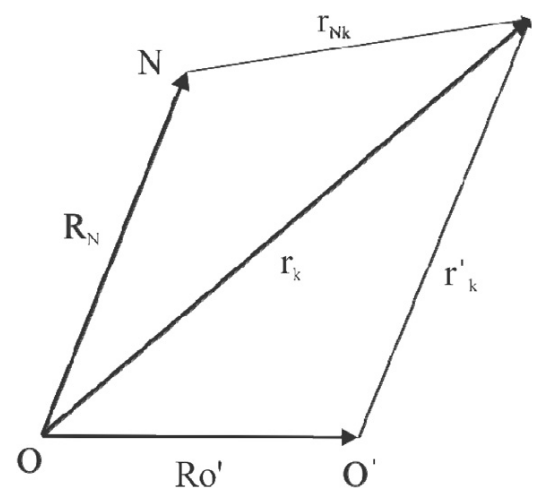
\includegraphics[width=0.3\textwidth]{origin_dependance_tensor.png}
\caption{Translation of the coordinate system for vector $\vec{Ro'}$. $\vec{R_N}$
  points to $N$-th atom, whereas small case $\vec r$ point to electrons  \cite{chemic_shift_tensor_review}.}
\end{wrapfigure}


  There are two contributions to the shielding tensor - paramagnetic and
  diamagnetic. The former is only present in materials with unpaired electrons
  and should not be confused with hyperfine tensor, also present in such materials.
  Diamagnetic contribution can be, in the first order of perturbation, calculated as \cite{chemic_shift_tensor_review}:
  \begin{equation}
    \sigma^d_{\alpha \beta}=\bra{\psi_0}\vec{r}_k \vec{r}_{Nk}\delta_{\alpha\beta}- \vec{r}_{k}\vec{r}_{Nk} \ket{\psi_0}
  \end{equation}
  and a similar expression holds also for paramagnetic contribution $\sigma^p_{\alpha\beta}$. Both
  expressions are nonlinear in $\vec r$. This seems to suggest that the values
  depend on the origin. It turns out, that the sum of both contributions does
  not depend on the origin, but only when one uses complete set of basis functions,
  which, in practice, is almost never the case. This is a serious problem
  because the terms that should theoretically cancel out have nontrivial
  contribution \cite{chemic_shift_tensor_review}. The issue is exaggerated by
  the fact that diamagnetic and paramagnetic contributions are of a different
  perturbation order.

  In contrast to shielding tensor, which depends only on electron density,
  hyperfine tensor depends on spin density \cite{calcul_hyper_tensor_param_nmr}.
  The anisotropic part of the tensor, also called Fermi contact term, is
  calculated as follows:
  \begin{equation}
    A_{iso}=\frac{4\pi}{6c^2}g_eg_N\beta_N\langle S_z \rangle \rho^{beta-alpha}(0),
    \end{equation}
where $g_e$ and $g_n$ are electronic and nuclear g-factors, $\langle S_z
\rangle$ is the expectation value of z component of total spin.
$\rho^{beta-alpha}$ is the difference between spin up and spin down electron
densities. Fermi contact term stems from magnetic dipole interaction between unpaired electron and nucleus. Dipole dipole interaction
also has anisotropic contribution to tensor, which is called dipolar term. Higher
order contributions are caused by the relativistic effects.
Relative sizes of hyperfine and chemical shifts vary greatly depending on
electronic configuration of molecule, however,
hyperfine shifts can reach much larger values than chemical shifts. 

\section{Purpose}
The purpose of this work and the follow on work associated with phd thesis, is to
systematically test various approaches and computational packages. Since MOFs
are crystalline materials one can choose periodic boundary conditions. The other
options is to use large cut-out of crystal structure and non-periodic boundary conditions to calculate
electronic structure. In the latter case one need to add atoms at the
boundaries, so that one does not end up with radicals. Of course, the former
approach also has downsides. These are mainly associated with the use of plane
waves as basis sets and their inability to fit steep, multi nodal, high angular
momentum states of $d$ shell electrons. For the same reason, the inner electrons
are often replaced by pseudo wave function, also called pseudopotential.
Although pseudopotentials are carefully constructed, they still represent an
approximation which may yield significant inaccuracies.

The other source of inaccuracies is the DFT method itself. Depending on
exchange---correlation functional used, one may obtain very different results.
The self interaction error of common dft poses a significant error especially
for metals, where valence electrons get over delocalized, causing large error in
electron density and thus also NMR parameters. To conclude this seminar, we are
attaching examples of two MOFs, for which NMR parameters were measured and
calculated. One is already discussed HKUST-1 and the other consists of central
copper ion and two molecules of acetil---acetonat.
\\

\begin{minipage}[]{0.6\linewidth}
  \centering 
  \begin{tabular}{|c ||c| c| c| c| c|}  \hline
    \multicolumn{6}{|c|}{ $\mathrm{Cu-(acetilacetonat)_2}$ } \\ \hline
  & \multicolumn{2}{|c|}{QE: PBE} & \multicolumn{2}{|c|} {ORCA: PBE0} &   \\ \hline
  C & $\delta^{cs} $ &  $\delta^{tot}$ & $\sigma^{cs} $ &  $\delta^{tot}$ & eks. \\ \hline
  4 & 118  & 59  & 109   & 80  & 108   \\ \hline
  6 & 37  & 270   & 30 & 199    & -53 \\ \hline
  10 & 209  & 199   & 196 & 186  & 97  \\ \hline
  \end{tabular}
  \captionof{table}{This is an example of a molecule where calculations differ
    significantly from experiments. Using two different computational packages
    and two completely different approaches yields quite similar results, but
    unfortunately both are quite far from the measurements.}
\end{minipage}%
\hspace{0.5cm}
\begin{minipage}[]{0.4\linewidth}
  \centering
  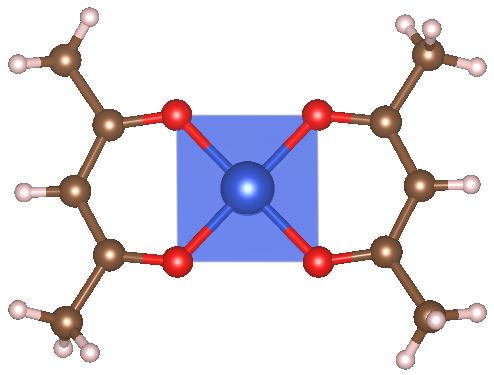
\includegraphics[width=0.8\textwidth]{cu-acac.jpeg}.
  \captionof{figure}{A molecule of $\mathrm{Cu-(acetilacetonat)_2}$.}
  \label{cu_acac}
\end{minipage}

\vspace{0.5cm}

\begin{minipage}[]{1.0\linewidth}
  \centering 
  \begin{tabular}{|c ||c| c| c| c| c| c| c|}  \hline
    \multicolumn{8}{|c|}{HKUST - 1} \\ \hline
  & \multicolumn{2}{|c|}{PBE}   &  \multicolumn{2}{|c|}{PBE0}   & \multicolumn{2}{|c|}{TPSS0} &  \\ \hline
  C & $\delta^{cs} $ &  $\delta^{tot}$  & $\delta^{cs} $  &  $\delta^{tot}$  & $\delta^{cs} $  &  $\delta^{tot}$ & eks. \\ \hline
  36 & 178  & -171.3 & 175 & -76.5 & 171 & -81.2 & -50  \\ \hline
  37 & 140  & 1028.4 &  134 & 802.7 & 130 & 798.2 & 853   \\ \hline
  38 & 138  & 299.8 & 138 & 218.6 & 136 & 216.6 &  228  \\ \hline
 \end{tabular}
 \captionof{table}{HKUST-1 calculation data compared to experimental values. The
 values are quite close for both hybrid functionals - PBE0 and TPSS0. Gga
 fucntional PBE fared much worse.}
\end{minipage}

\newpage \phantomsection


\addcontentsline{toc}{section}{Literatura}
\bibliographystyle{../myapsrevSLO}
\bibliography{../mybib}

\end{document}